% Copyright 2004 by Till Tantau <tantau@users.sourceforge.net>.
%
% In principle, this file can be redistributed and/or modified under
% the terms of the GNU Public License, version 2.
%
% However, this file is supposed to be a template to be modified
% for your own needs. For this reason, if you use this file as a
% template and not specifically distribute it as part of a another
% package/program, I grant the extra permission to freely copy and
% modify this file as you see fit and even to delete this copyright
% notice. 

\documentclass{beamer}

\usepackage{xcolor}
\usepackage{CJKutf8}
\usepackage{rotating}
\usepackage{subfigure}
\usepackage{graphicx}
\usepackage{algorithm}
\usepackage{algorithmicx}
\usepackage{amsmath}
\usepackage{amssymb}
\usepackage[noend]{algpseudocode}
\usepackage{wallpaper}
\algdef{SE}[DOWHILE]{Do}{DoWhile}{\algorithmicdo}[1]{\algorithmicwhile\ #1}%
\renewcommand{\algorithmicrequire}{\textbf{Input:}}
\renewcommand{\algorithmicensure}{\textbf{Output:}}
\newcommand{\var}[1]{\text{\texttt{#1}}}
\newcommand{\func}[1]{\text{\textsl{#1}}}


% table
\usepackage[normalem]{ulem}
\useunder{\uline}{\ul}{}
\usepackage{multirow}
\usepackage{tabularx}

\algdef{SE}[DOWHILE]{Do}{DoWhile}{\algorithmicdo}[1]{\algorithmicwhile\ #1}%

\usetheme{Madrid} % origin
\setbeamercolor{structure}{fg=violet}

\author{Chi-Ming~Lee}

\institute[NTHU EE] % (optional, but mostly needed)
{
    Department of Electrial Engineering\\
    National Tsing Hua University
}

\date{\today}

\AtBeginSubsection[]
{
    \begin{frame}<beamer>{Outline}
        \tableofcontents[currentsection,currentsubsection]
    \end{frame}
}

\begin{document}
\setbeamertemplate{background canvas}{\CenterWallPaper{.30}{./assets/nthu_watermark.eps}}
\begin{CJK}{UTF8}{bkai}

    \title[DeAr DSP]{ DeAr: 適用於異質系統架構之高效率且彈性的數位訊號處理器設計}
    \subtitle{DeAr: An Efficient and Flexible Digital Signal Processor Design for Heterogeneous System Architecture}

    \begin{frame}
        \titlepage
    \end{frame}

    \begin{frame}{Outline}
        \tableofcontents
        % You might wish to add the option [pausesections]
    \end{frame}

    % Section and subsections will appear in the presentation overview
    % and table of contents.

    \section{Introduction}

    \subsection{Motivation}

    \begin{frame}{Motivation (1/2)}
        \begin{itemize}
            \item {
                    The evolution of wireless communication standard drives the quest on a new DSP architecture.
                }
            \item {
                    E.g., LTE-A demands 10 times transmission rate than that of LTE.
                    \begin{itemize}
                        \item {
                                More sophisticated arithmetics are needed (throughput).
                            }
                        \item {
                                Algorithms for demodulation need to evolve rapidly (flexibility).
                        }
                        \item {
                                Endurance of embedded devices still matters (power-efficiency).
                        }
                    \end{itemize}
                }
            \item{ 
                    DSP has gone beyond the scalar architecture to increase throughput!
                    \begin{itemize}
                        \item Very Long Instruction Word architecture (VLIW)
                        \item Application Specific Instruction-set Processor (ASIP)
                    \end{itemize}
                }
            \item {
                    Unfortunately, VLIW and ASIP are opposite extreme cases...
                    \begin{itemize}
                        \item VLIW: good flexibility and bad power-efficiency
                        \item ASIP: good power-efficiency and bad flexibility
                    \end{itemize}
                }
            \item \large{\textbf{Achieving both of them is a challenge!}}
        \end{itemize}
    \end{frame}

    \begin{frame}{Motivation (2/2)}
        \begin{itemize}
            \item {
                    Heterogeneous computing, a system with multiple types of processors, is gaining momentum.
                    \begin{itemize}
                        \item {
                                CPU handles control-intensive tasks and coordinate cores.
                            }
                        \item {
                                DSP, GPU and FPGA handles data-intensive tasks for acceleration.
                            }
                        \end{itemize}
                }
            \item {
                    Industry standard for heterogeneous computing, \textit{Heterogeneous System Architecture} emerged in 2012.
                    \begin{itemize}
                        \item {
                                Proposed by leading semiconductor companies, AMD, ARM, MediaTek, Samsung etc, 
                            }
                        \item {
                                It has opened a new era for embedded computing platforms.
                            }
                        \end{itemize}
                }
            \item
                Shall make our new DSP architecture be compatible with HSA!
            \item
                \large{\textbf{A TIGER WITH WINGS}}
        \end{itemize}
    \end{frame}


    \subsection{Contribution}

    \begin{frame}{Contribution}
        \begin{itemize}
            \item {
                    We present \textbf{Dual-thread Architecture} (\textbf{DeAr}) DSP, which achieves both power-efficiency and flexibility.
                    \begin{itemize}
                        \item {
                                The multi-issue datapath manipulating Simultaneous Multi-threading.
                            }
                        \item {
                                Multi-banked register file (RF) with implicit RF addressing.
                            }
                        \item {
                                Transport-triggered data bus for exhaustive data forwarding.
                            }
                        \end{itemize}
                }
            \item {
                    A novel scheduling algorithm, HDFG-based scheduling is proposed.
                    \begin{itemize}
                        \item Going beyonds the conventional data flow graph (DFG) analysis.
                        \item Optimizing \textbf{power dissipation}, \textbf{flexibility} and \textbf{Operations per Cycle} (OPC).
                    \end{itemize}
                }
            \item {
                    We also propose a framework to integrate DeAr DSP with HSA.
                    \begin{itemize}
                        \item {
                                HSA compatible system integration framework.
                            }
                        \item {
                                HSA compatible compilation framework.
                            }
                        \end{itemize}
                }
            \item{
                    Compared with VLIW and ASIP respectively, DeAr saves: 
                    \begin{itemize}
                        \item {
                                \textbf{20.3\%--13.1\%} and \textbf{31.8\%--2.2\%} of power.
                            }
                        \item {
                                \textbf{36.1\%--31.5\%} and \textbf{28.2\%--5.7\%} of area.
                            }
                        \end{itemize}
                }
        \end{itemize}
    \end{frame}

    \section{Background}
    \subsection{Common DSP architectures}
    \begin{frame}{Very Long Instruction Word (VLIW)}
       \begin{columns}
           \begin{column}{0.4\textwidth}
               \begin{figure}[!ht]
                   \centering
                   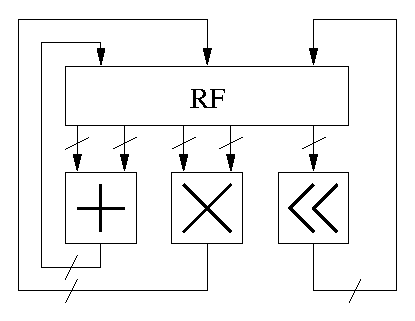
\includegraphics[width=0.9\textwidth]{./figs/vliw.eps}
                   \caption{VLIW example}
               \end{figure}
           \end{column}
           \begin{column}{0.6\textwidth}
              \begin{itemize}
                  \item Each function unit (FU) works independently with dedicated ports in RF (worst-case port count).
                  \item Pros:
                      \begin{itemize}
                          \item Multi-issue datapath \\ $\implies$ high OPC
                          \item Orthogonality among FUs \\ $\implies$ Good flexibility
                      \end{itemize}
                 \item Cons:
                     \begin{itemize}
                         \item Large port count in RF \\ $\implies$ Severe cost in power and area
                     \end{itemize}
              \end{itemize} 
           \end{column}
       \end{columns} 
    \end{frame}

    \begin{frame}{Application Specific Instruction Set Processor (ASIP)}
        \begin{columns}
            \begin{column}{0.4\textwidth}
                \begin{figure}[!ht]
                    \centering
                    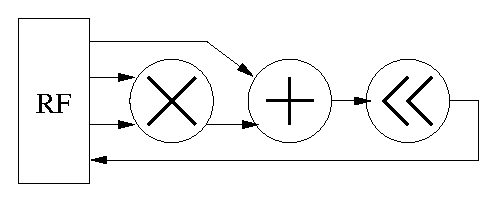
\includegraphics[width=0.9\linewidth]{./figs/cascade.eps}
                    \caption{ASIP example}
                \end{figure}
            \end{column}
            \begin{column}{0.6\textwidth}
               \begin{itemize}
                   \item FUs are configured or cascaded in a special manner (special-case port count).
                   \item Pros:
                       \begin{itemize}
                           \item Multi-issue datapath \\ $\implies$ high OPC
                           \item Medium port count in RF \\ $\implies$ Acceptable cost in power and area
                           \item Inherent forwarding path between FUs \\ $\implies$ Reducing cost in power
                       \end{itemize}
                   \item Cons:
                       \begin{itemize}
                           \item Fitting particular applications only \\ $\implies$ Poor flexibility
                       \end{itemize}
               \end{itemize} 
            \end{column}
        \end{columns} 
    \end{frame}
    %\begin{frame}{Transport-triggered Architecture (TTA)}
    %    \begin{itemize}
    %        \item foo
    %        \item bar
    %    \end{itemize}
    %    \begin{figure}[!ht]
    %        \centering
    %        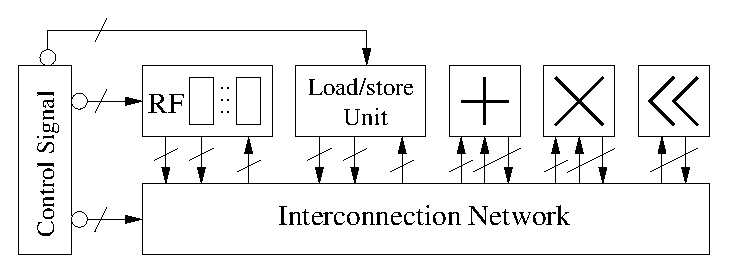
\includegraphics[width=0.6\linewidth]{./figs/tta.eps}
    %        \caption{TTA example}
    %    \end{figure}
    %\end{frame}

    \subsection{Heterogeneous System Architecture}
    \begin{frame}{Key Concepts of HSA}
       \begin{itemize}
           \item Heterogeneous multi-core platform
               \begin{itemize}
                   \item Particular processors handles particular tasks --- better power efficiency
               \end{itemize}
           \item Heterogeneous System Architecture Intermediate Language (HSAIL)
               \begin{itemize}
                   \item Providing an unified programming language of heterogeneous cores
                   \item Single Program Multiple Data (SPMD) programming model
               \end{itemize}
           \item Shared Virtual Memory (SVM)
               \begin{itemize}
                   \item Eliminating redundant transfer among cores
                   \item Passing pointers instead --- alleviating communication overhead
               \end{itemize}
           \item Architectural Queuing Language (AQL)
               \begin{itemize}
                   \item Handshaking protocol for cores
                   \item Task dispatching, information exchanging, synchronization, etc.
               \end{itemize}
       \end{itemize} 
    \end{frame}

    \begin{frame}{HSA Platform Example}
        \begin{figure}[!ht]
            \centering
            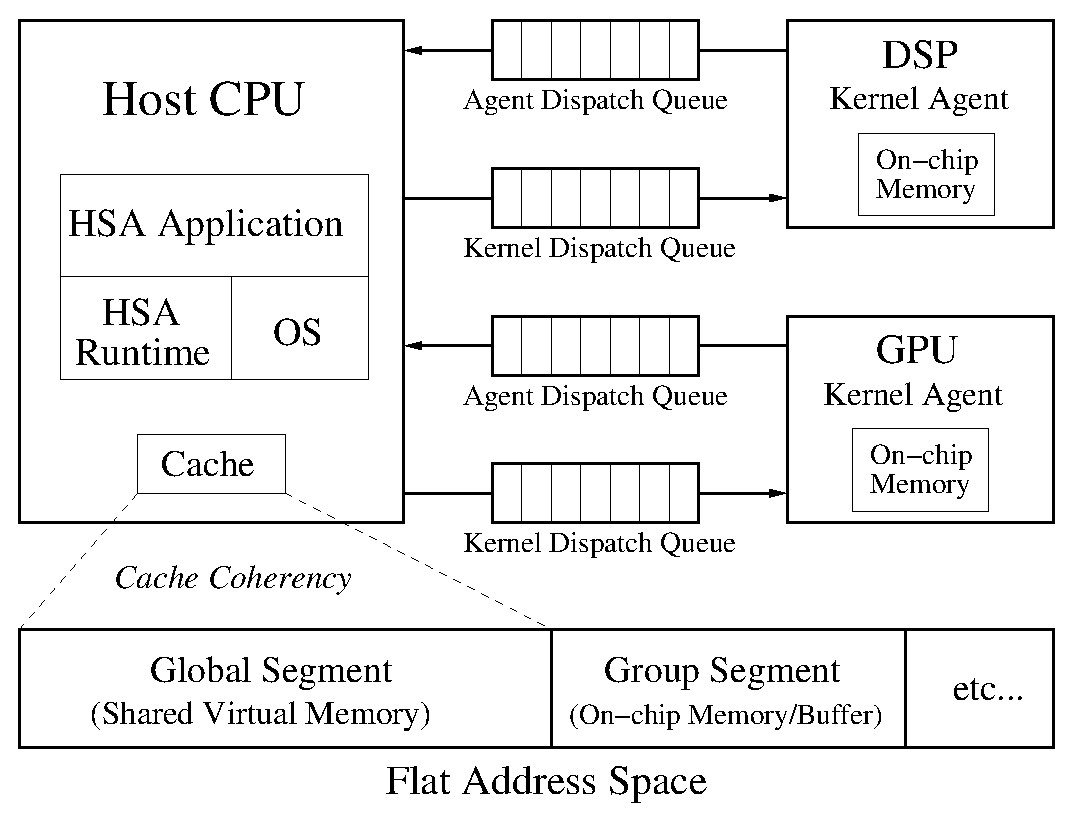
\includegraphics[width=0.8\textwidth]{./figs/systemspec.eps}
            \label{fig:systemspec}
        \end{figure}
    \end{frame}

    \begin{frame}{Execution Hierarchy}
        \begin{itemize}
            \item Work-item: the finest execution unit with dedicated registers.
            \item Work-group: a set of work-items sharing local memory (on-chip buffer)
            \item Grid: Assembly of all work-items and work-groups in the program context.
        \end{itemize}
        \begin{figure}[!ht] 
            \centering
            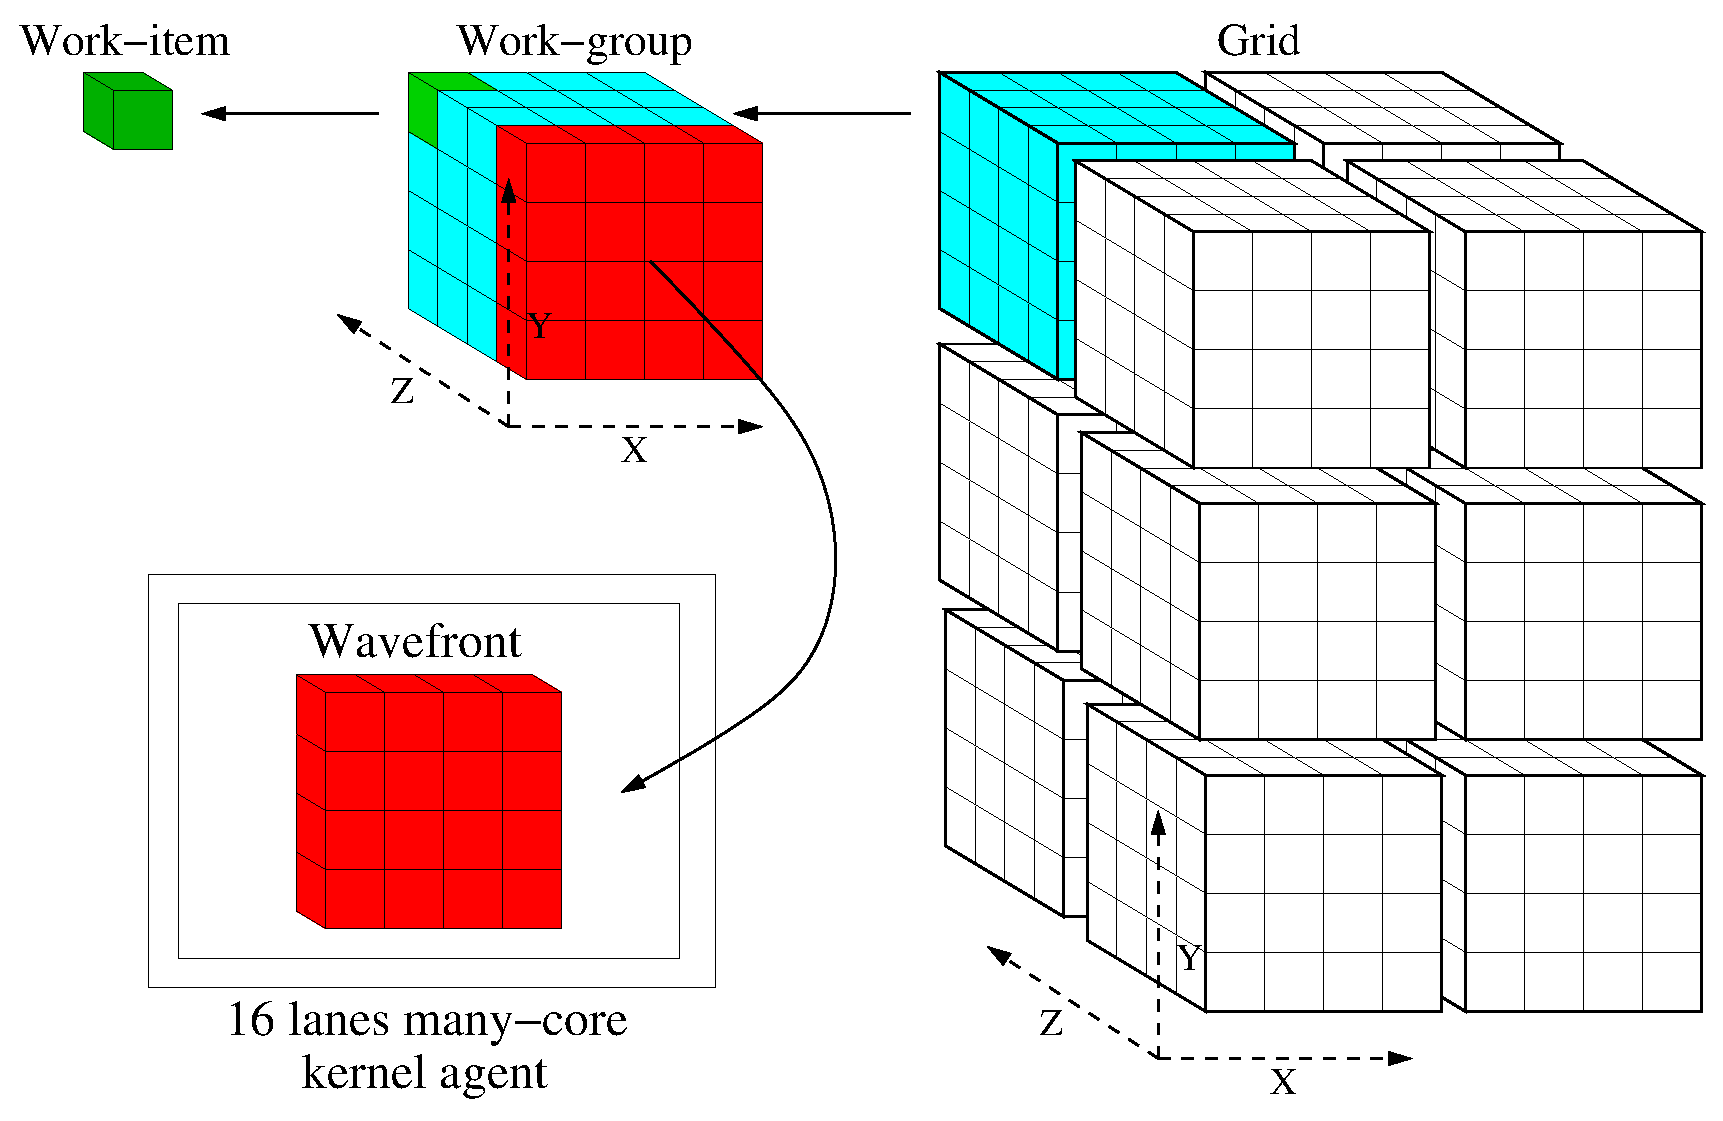
\includegraphics[width=0.7\textwidth]{./figs/grid.eps}
            \label{fig:grid}
        \end{figure}
    \end{frame}

    \begin{frame}{Software Infrastructure of HSA}
        \begin{figure}[!ht] 
            \centering
            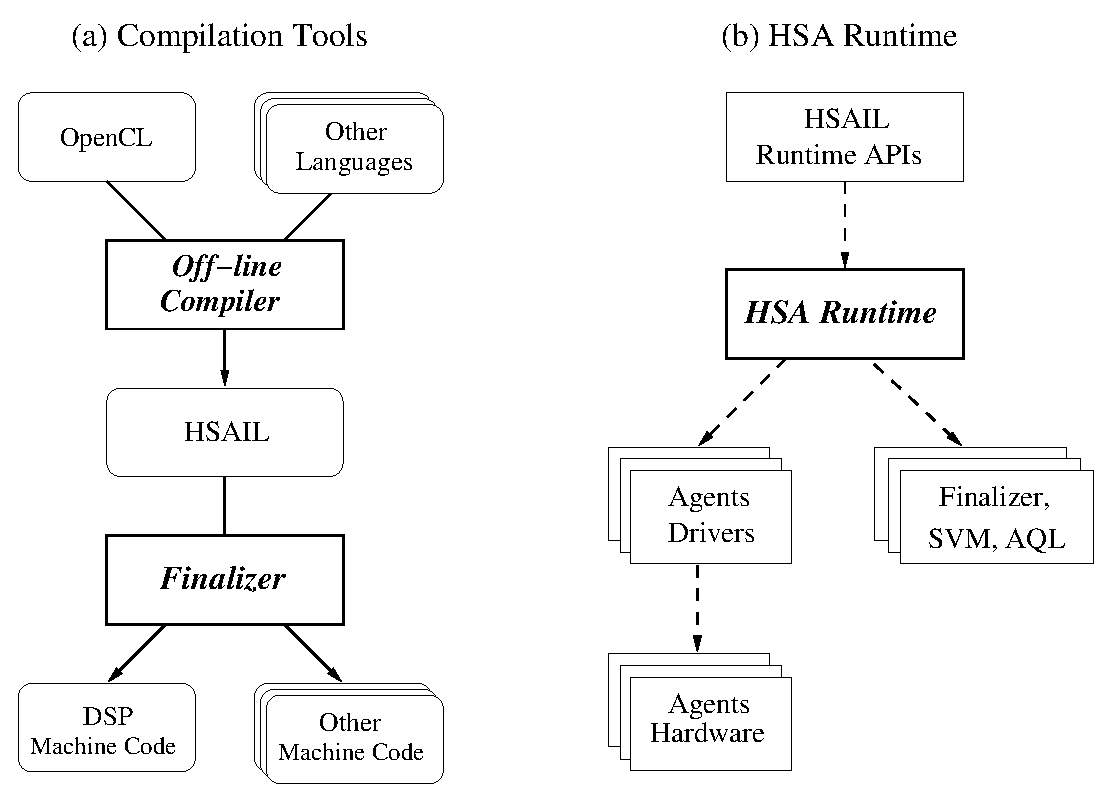
\includegraphics[width=0.8\textwidth]{./figs/swinf.eps}
            \label{fig:swinf}
        \end{figure}
    \end{frame}


    \section{Design and Implementation}
    \subsection{Proposed Architecture}

    \begin{frame}{System Integration (1/2)}
        \begin{columns}
            \begin{column}{0.6\textwidth}
                \begin{figure}[!ht] 
                    \centering
                    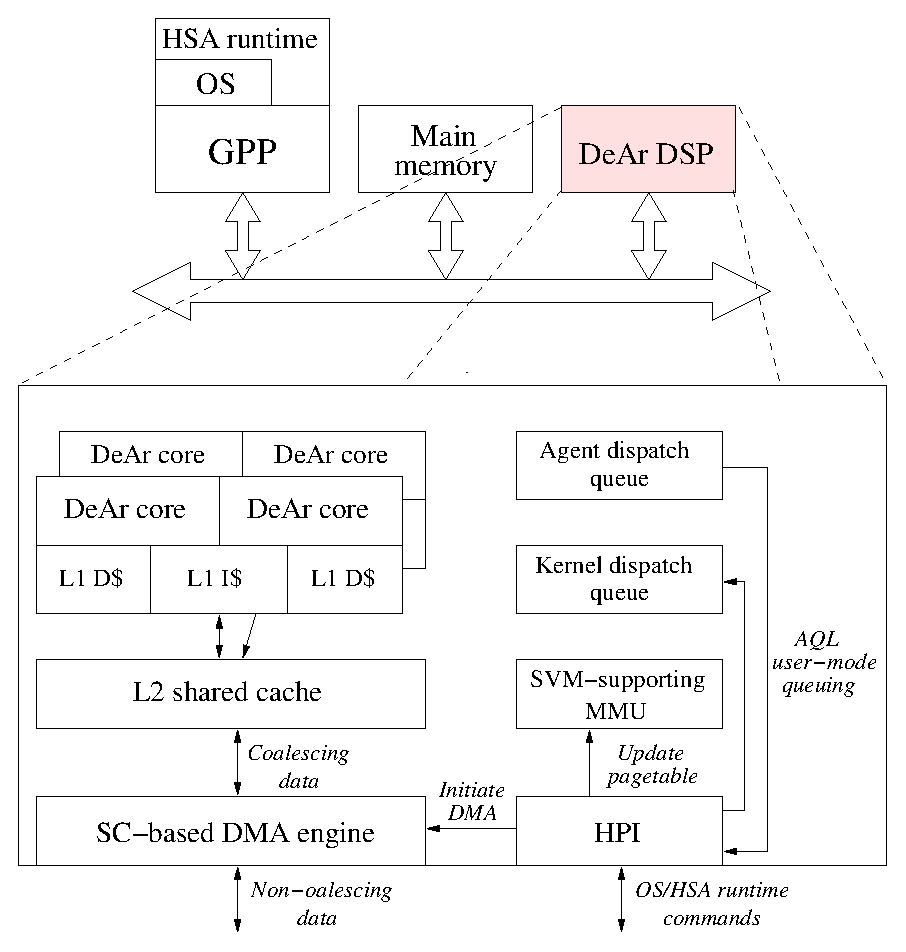
\includegraphics[width=1.0\textwidth]{./figs/archi.eps}
                    \label{fig:archi}
                \end{figure}
            \end{column}
            \begin{column}{0.4\textwidth}
            Key components:
                \begin{itemize}
                    \item Host port interface~\cite{hpi}
                    \item SC-based DMA engine~\cite{sc}
                    \item Shared L1 program cache~\cite{kelly2004shared}
                \end{itemize}
            \end{column}
        \end{columns}
    \end{frame}

    \begin{frame}{System Integration (2/2)}
        \begin{itemize}
            \item Host port interface (HPI)
                \begin{itemize}
                    \item Enabling host direct access to DeAr
                    \item Offloading MMU, AQL and SC control overhead to host
                \end{itemize}
            \item SC-based DMA engine
                \begin{itemize}
                    \item Initiating data transfer and transforming data layout on-the-fly
                    \item Improving data locality in DeAr --- coalescing access
                \end{itemize}
            \item Shared L1 program cache --- fitting SPMD programming model
        \end{itemize}
    \end{frame}

    \begin{frame}{Concepts for Acceleration}
        Key: Offloading a work-item to two DeAr threads.\\
        \begin{figure}[!ht]
            \begin{center}
                \subfigure[Execution flow of an HSA work-item]
                {
                    \label{fig:bb:1}
                    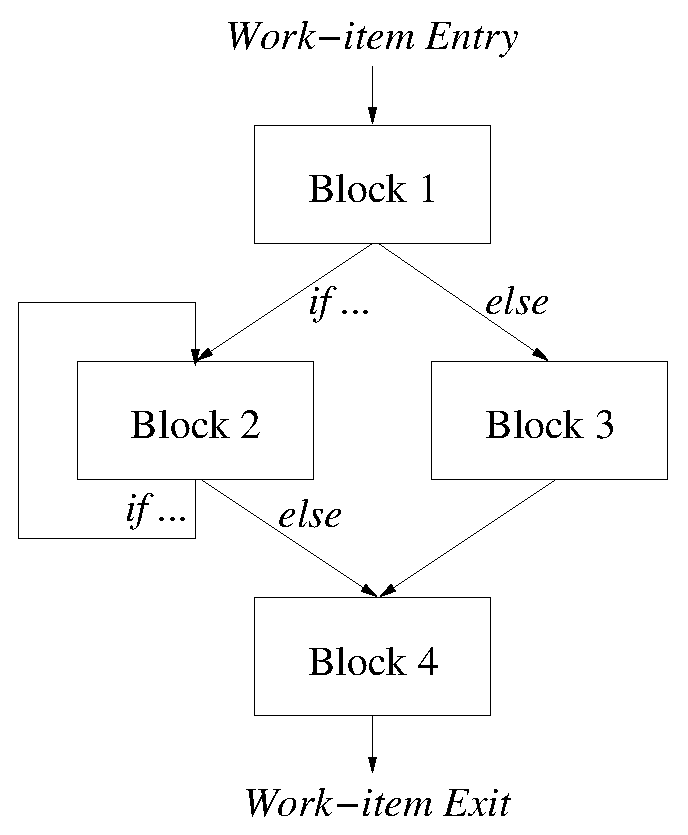
\includegraphics[width=0.33\textwidth]{figs/bb.eps}
                }
                \hfill
                \subfigure[Accelerating the execution of a Basic block]
                {
                    \label{fig:bb:2}
                    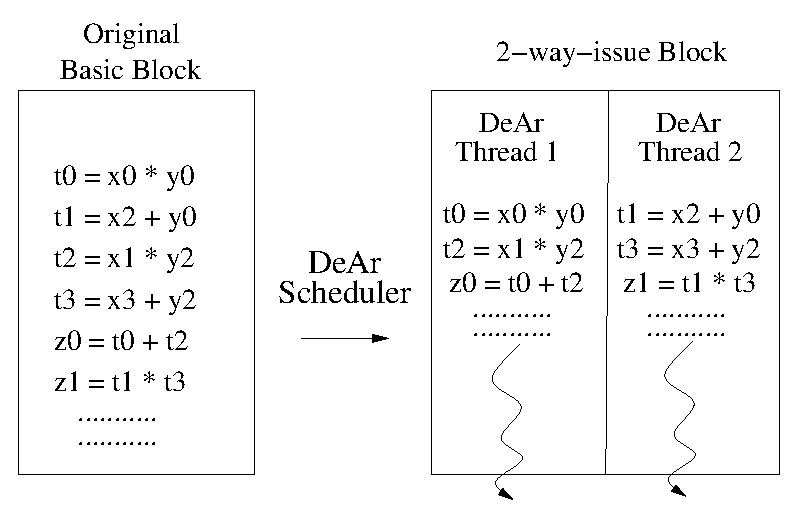
\includegraphics[width=0.55\textwidth]{figs/bb2.eps}
                }
            \end{center}
            \caption{Accelerating HSA with DeAr}
            \label{fig:bb}
        \end{figure}
    \end{frame}

    \subsection{Hardware Design and Implementation}
    \begin{frame}{Micro-architecture (1/2)}
        \begin{columns}
            \begin{column}{0.6\textwidth}
                \begin{figure}[!ht] 
                    \centering
                    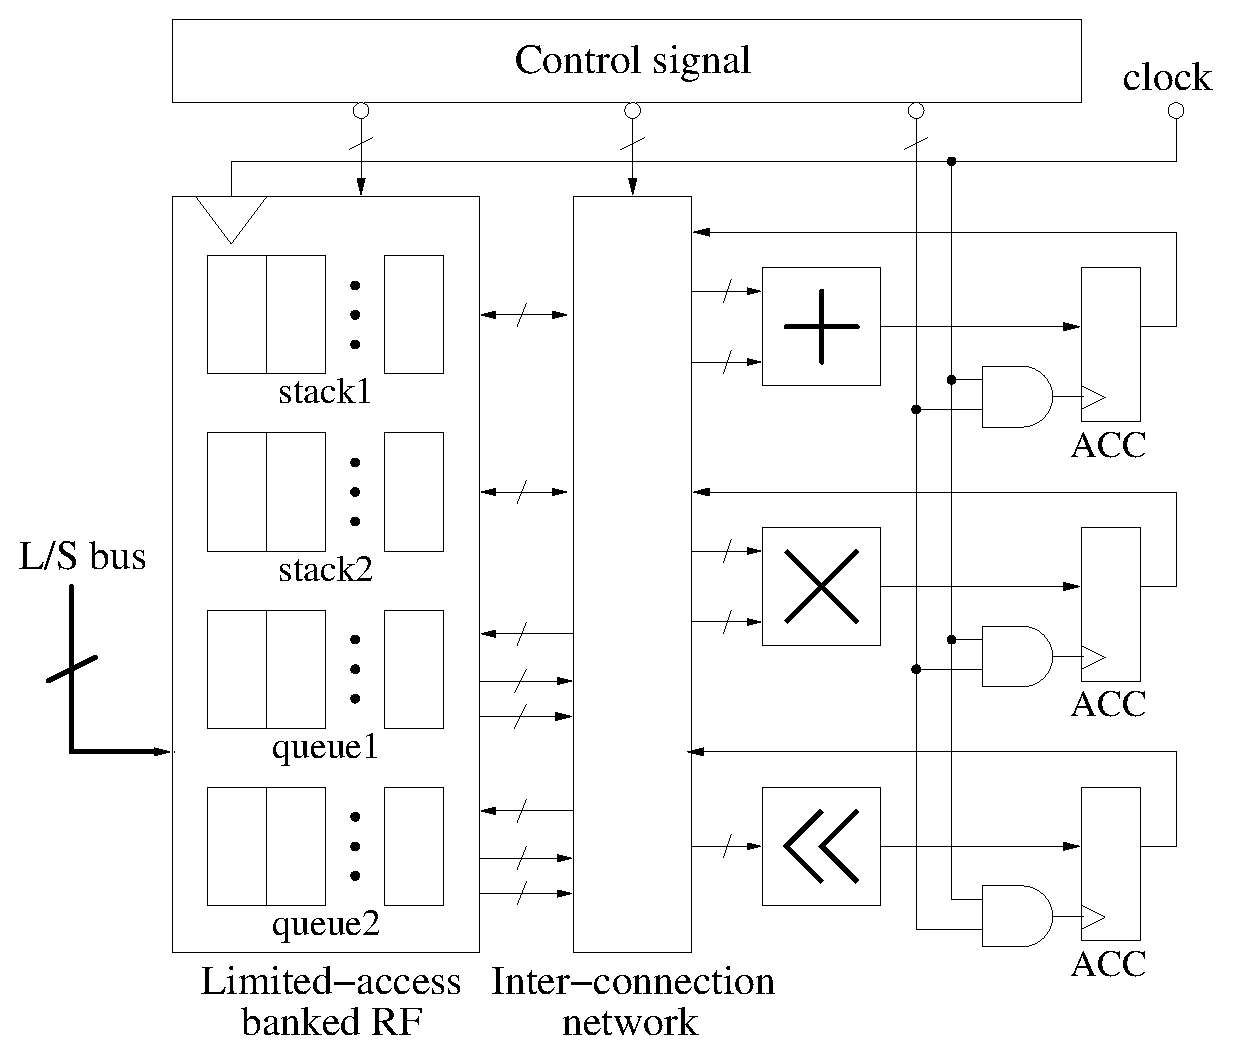
\includegraphics[width=1.0\textwidth]{./figs/micro.eps}
                \end{figure}
            \end{column}
            \begin{column}{0.4\textwidth}
                Key components:
                \begin{itemize}
                    \item Sequential-access Banked RF
                    \item Accumulator latches
                    \item Transport Triggered Data Bus
                \end{itemize}    
            \end{column}
        \end{columns}
    \end{frame}

    \begin{frame}{Micro-architecture (2/2)}
        \begin{itemize}
            \item Sequential-access Banked RF (SBRF)
                \begin{itemize}
                    \item Physical and symmetric separation for threads
                    \item Load/store queues buffer memory transfer data
                    \item Stack memory stores intermediate data
                    \item Implicit access reducing code size
                \end{itemize}
            \item Accumulator latches (ACCs) --- buffering arithmetic results for future reuse
            \item Transport-triggered Data Bus (TTDB)
                \begin{itemize}
                    \item Flexible data transport between ACCs and FUs
                    \item Facilitating exhaustive data reuse
                \end{itemize}
        \end{itemize}
    \end{frame}

    \begin{frame}{Instruction Set Architecture (1/2)}
        Each DeAr instruction is composed of two portions:
        \begin{itemize}
            \item Stack control portion: manipulating the stack memory
            \item RISC-fashion portion: a subset of common RISC ISA
        \end{itemize}
        \begin{table}[ht!]
            \centering
            \caption{Stack access portion of a DeAr instruction}
            \resizebox{0.9\textwidth}{!}
            {
                \begin{tabular}{|l|l|l|}
                    \hline
                    \multicolumn{1}{|c|}{\textbf{Name}} & \multicolumn{1}{c|}{\textbf{Meaning}} & \multicolumn{1}{c|}{\textbf{Note}} \\ \hline
                PUSH & \begin{tabular}[c]{@{}l@{}}1. Add the head address by 1\\ 2. Write the new data to the head address\end{tabular} & \multirow{2}{*}{ \parbox{5cm}{A "pop" followed by a "push" is equivalent to a "modify"} } \\ \cline{1-2}
                POP                               & \begin{tabular}[c]{@{}l@{}}1. Subtract the head address by 1\\ 2. Invalidate the previous head data\end{tabular} & \\ \hline
                    MODIFY                            & Modify the head data to to the new data & The head address remains \\ \hline
                    STALL                               & No operation & The head address and data remain \\ \hline
                \end{tabular}
            }
        \end{table}
    \end{frame}


    \begin{frame}{Instruction Set Architecture (2/2)}
        \begin{table}[ht!]
            \centering
            \caption{RISC-fashion portion of a DeAr instruction}
            \resizebox{0.8\textwidth}{!}
            {
                \begin{tabular}{|c|l|l|c|}
                    \hline
                    \multicolumn{1}{|c|}{\textbf{Category}} & \multicolumn{1}{c|}{\textbf{Name}} & \multicolumn{1}{c|}{\textbf{Meaning}} & \multicolumn{1}{c|}{\textbf{Target}} \\ \hline
                \multirow{7}{*}{ \begin{tabular}[c]{@{}l@{}} \\ A type \end{tabular}}      & ADD & \textbf{d} = \textbf{s} + \textbf{t}  & \multirow{7}{*}{\begin{tabular}[c]{@{}l@{}} \\ Datapath \end{tabular}}  \\ \cline{2-3}
                                                                                           & SUB & \textbf{d} = \textbf{s} $-$ \textbf{t} & \\ \cline{2-3} 
                                                                                           & MUL & \textbf{d} = \textbf{s} $\times$ \textbf{t} & \\ \cline{2-3} 
                                                                                           & SHL & \textbf{d} = \textbf{s} $<<$ \textbf{t} & \\ \cline{2-3}
                                                                                           & SHR & \textbf{d} = \textbf{s} $>>$ \textbf{t} & \\ \cline{2-3}
                                                                                           & MV  & \textbf{d} = \textbf{s} + 0 or \textbf{d} = \textbf{s} << 0 & \\ \cline{2-3} 
                                                                                           & NOP & \begin{tabular}[c]{@{}l@{}}1. disable write back \\ 2. clock-gate the accumulator \end{tabular}& \\ \hline
                \multirow{3}{*}{ \begin{tabular}[c]{@{}l@{}} \\ \\ B type \end{tabular}}          & JMP & pc = pc + \textbf{a}  & \multirow{3}{*}{ \begin{tabular}[c]{@{}l@{}} \\ \\ Instruction unit \end{tabular}} \\ \cline{2-3}
                                                                                                  & BZ  & \begin{tabular}[c]{@{}l@{}} \textit{if}(stack1.read() == stack2.read())\\ \ \ \ \ \ \ \ pc = pc + \textbf{a} \end{tabular} & \\ \cline{2-3}
                                                                                                  & BNZ & \begin{tabular}[c]{@{}l@{}} \textit{if}(stack1.read() != stack2.read())\\ \ \ \ \ \ \ \ pc = pc + \textbf{a} \end{tabular} & \\ \hline
                \multirow{2}{*}{ \begin{tabular}[c]{@{}l@{}} \\ M type \end{tabular}}           & LD  & \begin{tabular}[c]{@{}l@{}} \textit{repeat}(\textbf{r})\\ \ \ \ \ \ \ \ load\_queue.push (memory[\textbf{a}]) \end{tabular}& \multirow{2}{*}{\begin{tabular}[c]{@{}l@{}} \\  Load/store unit \end{tabular}} \\ \cline{2-3} 
                                                                                                & ST  & \begin{tabular}[c]{@{}l@{}} \textit{repeat}(\textbf{r})\\ \ \ \ \ \ \ \ memory[\textbf{a}] = store\_queue.pop() \end{tabular}& \\ \hline
                \end{tabular}
            }
        \end{table}
    \end{frame}

    \subsection{Software Design and Implementation}
    \begin{frame}{Software Framework}
        \begin{enumerate}
            \item Compilation
                \begin{itemize}
                    \item DeAr users program in high level languages (OpenCL or C++)
                    \item Off-line compiler~\ref{cloc} from HSA foundation compiles them to HSAIL
                \end{itemize}
            \item Finalization
                \begin{itemize}
                    \item Converting HSAIL to data flow graph (DFG)
                        \begin{itemize}
                            \item Reaching definition analysis (RDA)
                            \item Single static assignment (SSA)
                        \end{itemize}
                    \item Converting DFG to hierarchical data flow graph (HDFG)
                \end{itemize}
            \item HDFG-based scheduling
                \begin{itemize}
                    \item OPC optimization --- inter-tree and intra-tree parallelism
                    \item Power optimization --- exhaustive forwarding
                    \item Memory footprint optimization --- LIFO fashion and minimum stack consumption
                    \item Code generation
                \end{itemize}
        \end{enumerate}
    \end{frame}

    \begin{frame}{Finalization: Converting HSAIL to DFG}
               % \begin{algorithm}[H] \fontsize{10pt}{10pt}\selectfont  
        \begin{columns}
            \begin{column}{0.45\textwidth}
               \begin{block}{HSAIL: sum of products}
                   ld\_global\_u32 \$s2, [\$d0]; \\ 
                   ld\_global\_u32 \$s3, [\$d1]; \\ 
                   ld\_global\_u32 \$s2, [\$d2]; \\
                   ld\_global\_u32 \$s3, [\$d3]; \\
                   mul\_u32 \$s1, \$s2, \$s3; \\
                   mul\_u32 \$s4, \$s5, \$s6; \\
                   add\_u32 \$s7, \$s1, \$s4; \\
                   st\_global\_u32 \$s7, [\$d4]; \\
               \end{block} 
            \end{column}
            \begin{column}{0.55\textwidth}
                \begin{enumerate}
                    \item RDA retrieves use-define chains.
                    \item SSA renames variables.
                        \begin{itemize}
                            \item Give a new name to each LHS variable
                            \item Update corresponding RHS based on RDA
                        \end{itemize}
                    \item Re-traversing new code
                        \begin{itemize}
                            \item Store assignments in $V_{OP}$
                            \item Store dependencies in $E_{OP}$
                        \end{itemize}
                    \item DFG: $G = (V_{OP}, E_{OP})$ is obtained.
                        \begin{itemize}
                            \item Vertex: operation
                            \item Edge: data flow
                        \end{itemize}
                \end{enumerate}
           \end{column}
        \end{columns}
    \end{frame}

    \begin{frame}{Finalization: Converting DFG to HDFG}
        \begin{itemize}
            \item Conventional DSP program analysis: data flow graph (DFG) analysis
            \item We propose \textbf{Hierarchical data flow graph (HDFG)} \\
                    --- providing abundant information for optimizations
            \item After conversion, HDFG: $\bar{G} = (V_{BT}, E_{BT})$ is obtained.
                \begin{itemize}
                    \item Vertex: binary tree $BT$
                    \item Edge: data flow cross $BT$
                \end{itemize}
        \end{itemize}
        \begin{figure}[!ht]
            \begin{center}
                \subfigure[DFG example]
                {
                    \label{fig:dfg:dfg}
                    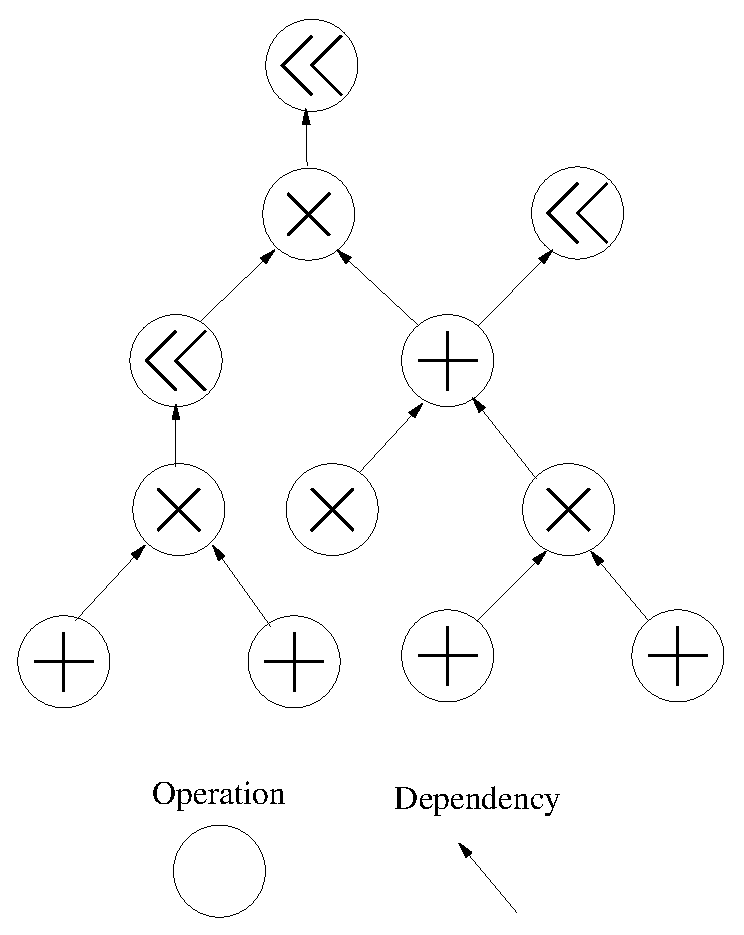
\includegraphics[width=0.35\textwidth]{figs/dfg.eps}
                }
                \subfigure[Corresponding HDFG]
                {
                    \label{fig:dfg:hdfg}
                    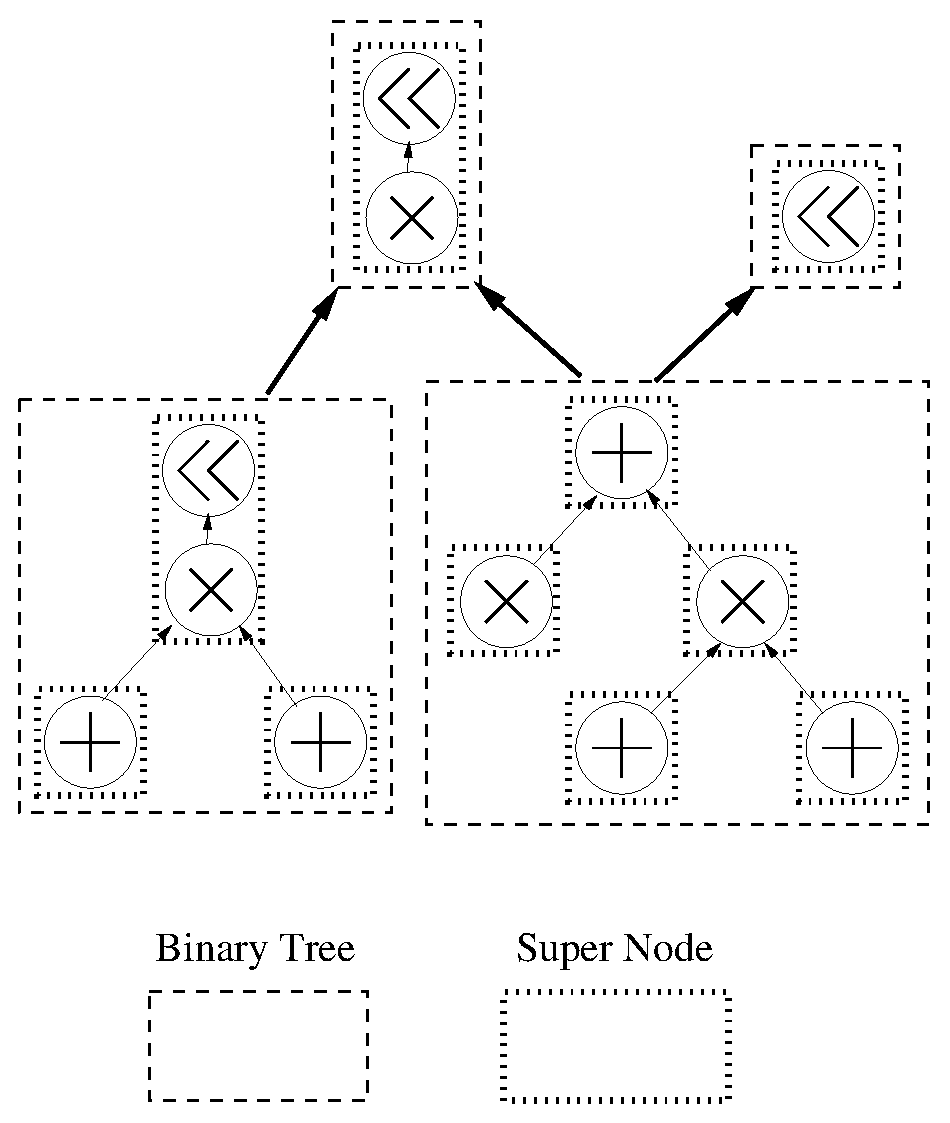
\includegraphics[width=0.35\textwidth]{figs/hdfg.eps}
                }
            \end{center}
        \end{figure}
    \end{frame}
    \begin{frame}{Compilation: Properties of HDFG}
        \begin{itemize}
            \item Cascaded or isolated $OP$ form $SN$ \\ --- data forwarding must performed within $sn$.
            \item Neighboring or isolated $sn$ form full binary tree $BT$ \\
                --- parent $SN$ receives data from stack and TTDB
                \begin{itemize}
                    \item First operand popped from stack
                    \item Second operand forwarded from TTDB
                \end{itemize}
                Within a $BT$, a parent $SN$ receives the first operand popped from the stack and the second one forwarded via TTDB.
            \item Dependencies among $SN$ that cross $BT$ are inherited
            \item After scheduled, $BT$ and its edges are erased from HDFG
        \end{itemize}
    \end{frame}



    \begin{frame}{HDFG-based scheduling: Inter-tree parallelism}
        \textbf{Achieving high OPC by exploring parallelism in HDFG}
        \begin{itemize}
            \item A $BT$ without in-edges is free to be scheduled to a thread
                \begin{itemize}
                    \item Operations in $BT$ are turned into a list
                    \item The thread executes operations on the list one by one
                \end{itemize}
            \item Two free $BT$s are \textbf{parallelizable} --- \textbf{inter-tree parallelism}
                \begin{itemize}
                    \item Processed by two threads respectively and concurrently.
                    \item Proceeding until all $BT$ are consumed
                \end{itemize}
        \end{itemize}
        But sometimes...
        \begin{itemize}
            \item Only one $BT$ exists in HDFG at beginning
            \item One $BT$ remains after scheduling
            \item One partial $BT$ remains after scheduling
        \end{itemize}
        \vspace{1em}
        \centering
        \textbf{Exploring intra-tree parallelism!}
    \end{frame}

    \begin{frame}{HDFG-based scheduling: Intra-tree parallelism}
        \begin{columns}
            \begin{column}{0.35\textwidth}
                
            \end{column}
            \begin{column}{0.65\textwidth}
                \begin{itemize}
                    \item Partitioning $bt$ into three parts --- root, left and right-subtrees
                        \begin{itemize}
                            \item Root: can only be handled sequentially
                            \item Left and right-subtrees --- \textbf{intra-tree parallelism}, processed by two threads concurrently
                        \end{itemize}
                    \item Imbalance subtree size lead to smaller $bt$ remaining after scheduling
                    \item Recursively partitioning and scheduling until completion
                \end{itemize} 
                \vspace{1em} 
                Parallelism is good, but how to handle ALU conflict?\\
                \vspace{1em} 
                \centering
                \textbf{DP-based ALU-allocation!}
            \end{column}
        \end{columns}
    \end{frame}

    \begin{frame}{HDFG-based scheduling: DP-based ALU-Allocation}
        \begin{itemize}
            \item Analyzing operation-lists of two threads by Dynamic programming (DP)
            \item DP determines which thread stalls at conflict, and achieved optimized OPC
            \item An example where two threads have MMMAAA in their operation-lists
        \end{itemize}
        \begin{figure}[!ht]
            \begin{center}
                \subfigure[Stage 1: scoring table modeling]
                {
                    \label{fig:alloc:1}
                    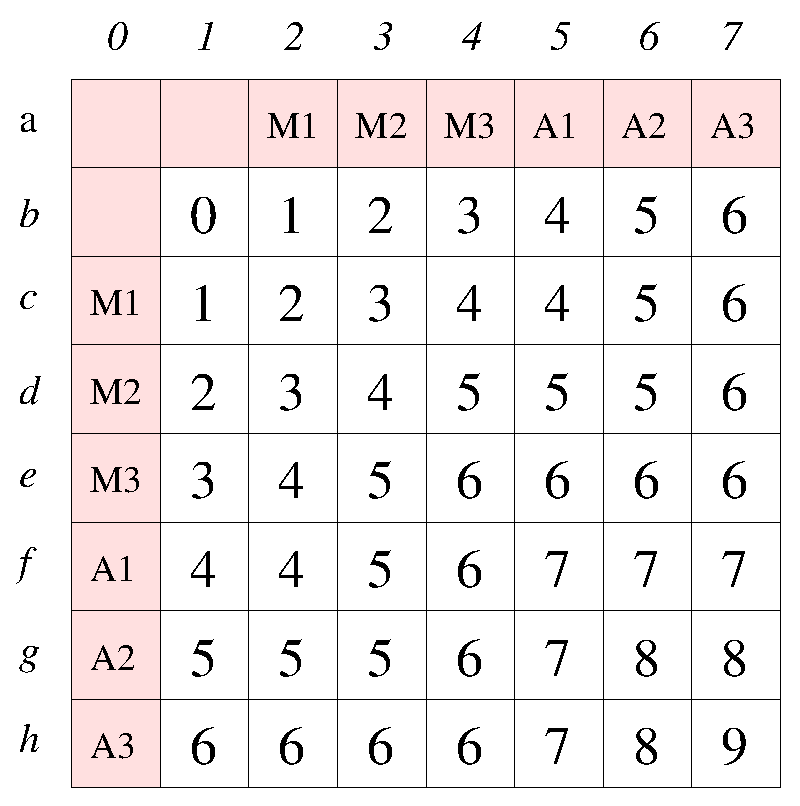
\includegraphics[width=0.3\textwidth]{figs/alloc.eps}
                }
                \hfill
                \subfigure[Stage 2: scoring table filling]
                {
                    \label{fig:alloc:2}
                    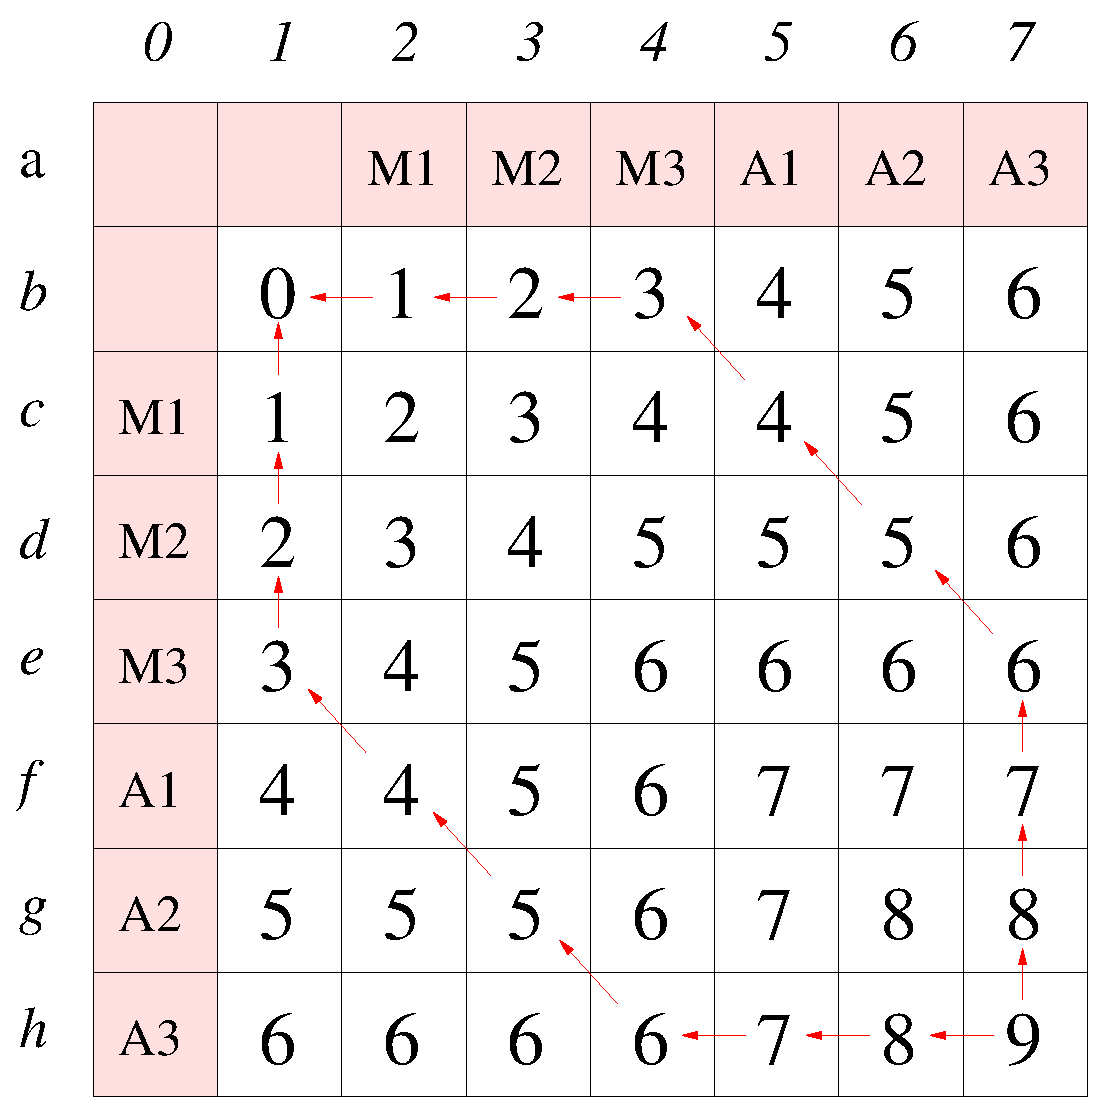
\includegraphics[width=0.3\textwidth]{figs/alloc2.eps}
                }
                \hfill
                \subfigure[Stage 3: backtracking]
                {
                    \label{fig:alloc:3}
                    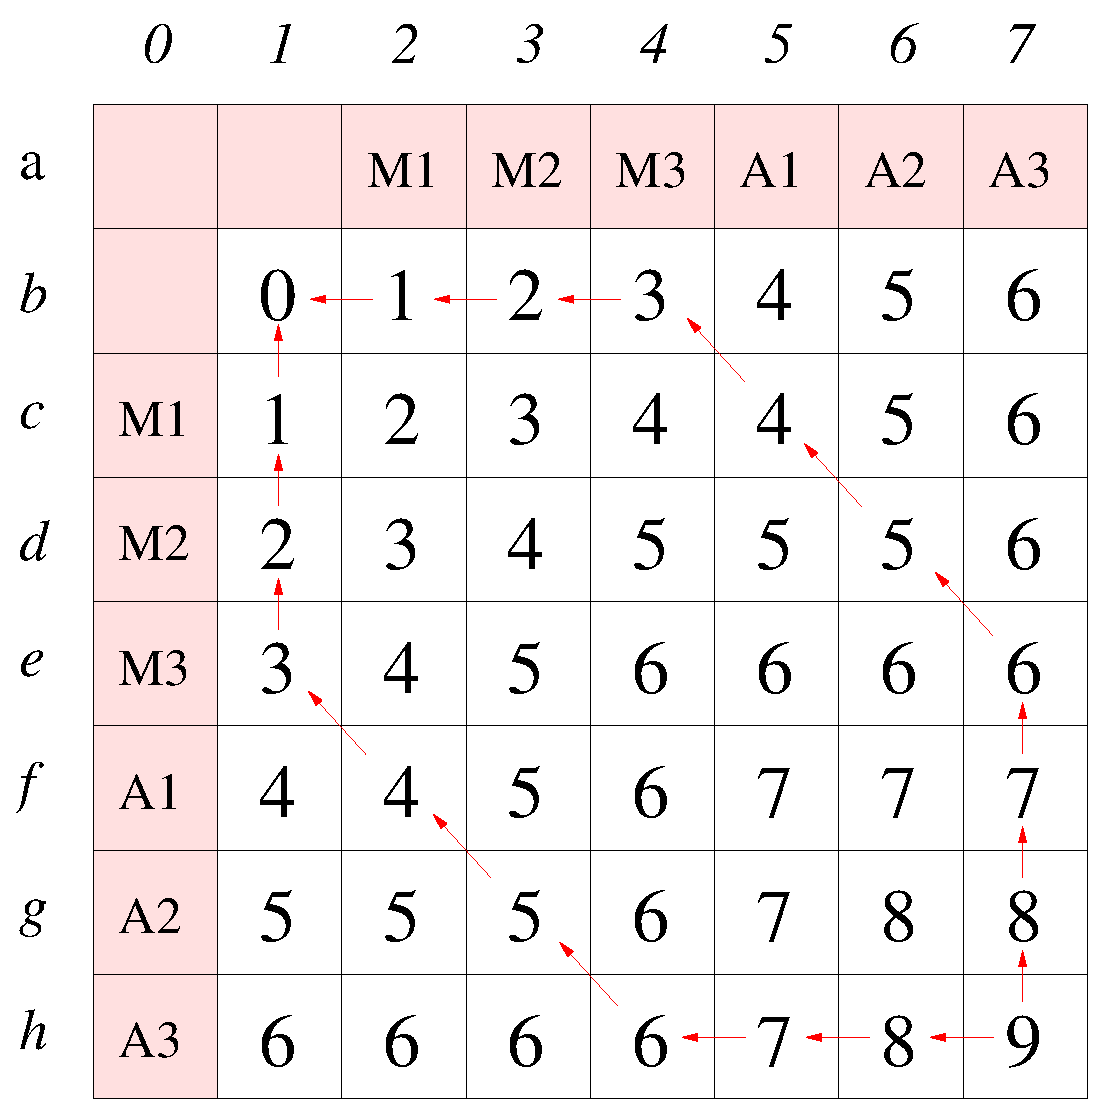
\includegraphics[width=0.3\textwidth]{figs/alloc3.eps}
                }
            \end{center}
            \label{fig:alloc}
        \end{figure}
    \end{frame}

    \begin{frame}{HDFG-based scheduling: HFPT sort}
        \begin{itemize}
            \item HFPT (higher-first post-order) sort determines exeuction order in $BT$
            \item Post-order traversal ensures LIFO memory footprint \\ --- \textbf{achieving flexibility}
            \item Higher-first strategy lets higher subtree go first \\ --- \textbf{minimizing stack consumption}
            \item $OP$s in $SN$ are atomic where data must flows via forwarding bus \\ -- \textbf{reducing power}
        \end{itemize}
        \begin{figure}[!h]
            \begin{center}
                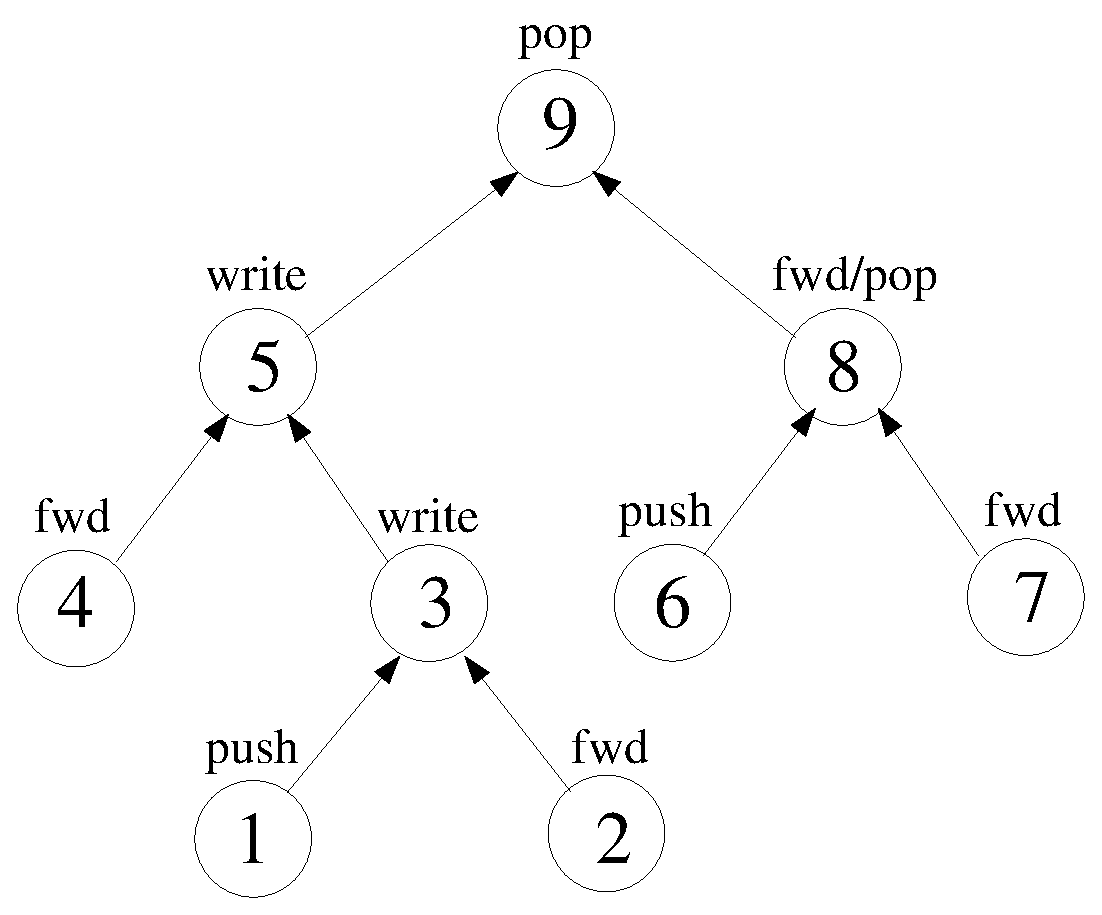
\includegraphics[width=0.4\textwidth]{figs/hfpt.eps}
            \end{center}
            \label{fig:hfpt}
        \end{figure}%
    \end{frame}

    \section{Performance Evaluation}
    \subsection{Experiment Setup}
    \begin{frame}{Why Single-core Evaluation?}
        \begin{itemize}
            \item Multi-core performance is highly correlated with issues not discussed in this work.
                \begin{itemize}
                    \item Core interconnection
                    \item Memory subsystem 
                    \item Shared memory or message passing
                \end{itemize}
            \item Programming language also plays a crucial role, but popular ones are still contending for becoming the standard. \\
                --- HSA, OpenCL, CUDA, OpenMP, etc.
            \item Benchmarking multi-core DSP is still an open field of study~\cite{landscape}
        \end{itemize}       
    \end{frame}
    \begin{frame}{Simulation Benchmark Suites}
        \begin{itemize}
            \item Three primitive operations --- addition, multiplication and shifting.
            \item BLAS --- classic matrix/vector library for wireless communication.
            \item GDSPK --- common DSP filters and transformations.
        \end{itemize}
        \begin{table}[!ht]
            \centering
            \resizebox{\columnwidth}{!}
            {
                \begin{tabular}{|c|c|c|c|c|c|c|c|c|}
                    \hline
                    \multicolumn{9}{|c|}{\textbf{Basic linear algebra subprograms (BLAS)}} \\ \hline
                    Benchmark              & AXPY   & MV     & MM      & INV      & CAXPY  & CMV  & CMM    & CINV  \\ \hline
                    \# add            &  32    &  56    &   48    &    75    &  128   & 132  &   90   &  88   \\ \hline
                        \# mul            &  32    &  64    &   64    &   172    &  128   & 144  &  108   & 114   \\ \hline
                        \# sht            &   0    &   0    &    0    &     0    &    0   &   0  &    0   &   0   \\ \hline
                        \# op             &  64    & 120    &  112    &   247    &  256   & 276  &  198   & 202   \\ \hline
                        \multicolumn{9}{|c|}{\textbf{General DSP kernels (GDSPK)}}                     \\ \hline
                        Benchmark              & FIR    & CFIR   & LPFIR   & Biquad   & IT     & DCT  & IMDCT  & FFT   \\ \hline
                        \# add            & 15     &  62    &   15    &    8     &  32    &  29  &   21   &  23   \\ \hline
                        \# mul            & 16     &  64    &    8    &    9     &   0    &  12  &   11   &  10   \\ \hline
                        \# sht            &  0     &   0    &    0    &    0     &  10    &   9  &    9   &   0   \\ \hline
                        \# op             & 31     & 126    &   23    &   17     &  42    &  50  &   41   &  33   \\ \hline
                    \end{tabular}
                }
            \end{table}
    \end{frame}

    \begin{frame}{Simulation Environment}
            \begin{itemize}
                \item DUT is replaced with \textbf{DeAr}, \textbf{scalar}, \textbf{VLIW} and \textbf{composite-ALU} (cascade-ALU ASIP) in accordance.
                \item Composite-ALU is evaluated with best two ALU configurations (MSA and AMS) respectively.
                \item Designs have compatible RF (32 cells) and ALU resources (one adder, multiplier and shifter).
            \end{itemize}
            \begin{figure}[!ht] 
                \centering
                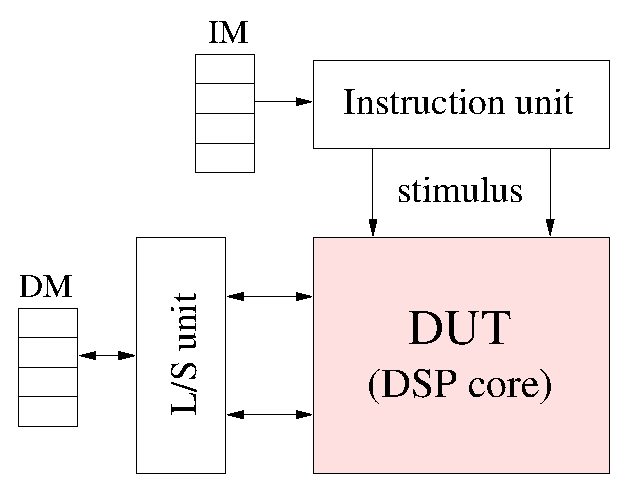
\includegraphics[width=0.45\textwidth]{./figs/sim.eps}
            \end{figure}
    \end{frame}

    \subsection{Pre-synthesis Analysis}

    \begin{frame}{Operations per Cycle}
        \begin{table}[!ht]
            \centering
            \resizebox{\columnwidth}{!}
            {
                \begin{tabular}{|c|c|c|c|c|c|c|c|c|c|}
                    \hline
                    \multicolumn{10}{|c|}{\textbf{Basic linear algebra subprograms (BLAS)}} \\ \hline
                    Benchmark  &  AXPY  &  MV  &  MM  &  MINV  &  CAXPY  &  CMV  &  CMM  &  CMINV  &  Average \\ \hline 
                    VLIW  &   1.94  &   1.85  &   1.72  &   1.44  &   1.97  &   1.89  &   1.80  &   1.76  &   1.79     \\ \hline 
                    DeAr  &   1.94  &   1.85  &   1.72  &   1.40  &   1.97  &   1.89  &   1.80  &   1.62  &   1.77     \\ \hline
                    Composite-MSA  &   2.00  &   1.88  &   1.75  &   1.37  &   1.33  &   1.35  &   1.38  &   1.53  &   1.57     \\ \hline 
                    Composite-AMS  &   1.00  &   1.00  &   1.00  &   1.02  &   1.00  &   1.00  &   1.00  &   1.04  &   1.01     \\ \hline 
                    Scalar  & 1.0  & 1.0  & 1.0  & 1.0  & 1.0  & 1.0  & 1.0  & 1.0  & 1.0 \\ \hline 
                    \multicolumn{10}{|c|}{\textbf{General DSP application kernels (GDSPK)}}                     \\ \hline
                    Benchmark  &  FIR  &  CFIR  &  LPFIR  &  Biquad  &  IT  &  DCT  &  IMDCT  &  FFT  &  Average \\ \hline 
                    VLIW  &   1.82  &   1.91  &   1.67  &   1.55  &   1.33  &   1.61  &   1.86  &   1.38  &   1.64     \\ \hline 
                    DeAr  &   1.82  &   1.91  &   1.67  &   1.55  &   1.33  &   1.47  &   1.46  &   1.32  &   1.57     \\ \hline 
                    Composite-MSA  &   1.94  &   1.34  &   1.44  &   1.42  &   1.31  &   1.14  &   1.28  &   1.06  &   1.35     \\ \hline 
                    Composite-AMS  &   1.00  &   1.00  &   1.53  &   1.21  &   1.14  &   1.61  &   1.52  &   1.27  &   1.29     \\ \hline 
                    Scalar  & 1.0  & 1.0  & 1.0  & 1.0  & 1.0  & 1.0  & 1.0  & 1.0  & 1.0 \\ \hline 
                \end{tabular}
            }
        \end{table}

    \end{frame}

    \begin{frame}{Register File Access Rate}
        \begin{table}[!ht]
            \centering
            \resizebox{\columnwidth}{!}
            {
                \begin{tabular}{|c|c|c|c|c|c|c|c|c|c|}
                    \hline
                    \multicolumn{10}{|c|}{\textbf{Basic linear algebra subprograms (BLAS)}} \\ \hline
                    Benchmark  &  AXPY  &  MV  &  MM  &  MINV  &  CAXPY  &  CMV  &  CMM  &  CMINV  &  Average \\ \hline 
                    DeAr  &   0.67  &   0.69  &   0.71  &   0.67  &   0.67  &   0.68  &   0.70  &   0.71  &   0.69     \\ \hline
                    Composite-MSA  &   0.67  &   0.69  &  0.71  &   0.82  &   0.83  &   0.83  &   0.82  &   0.77  &  0.77     \\ \hline 
                    Composite-AMS  &   1.0  &   1.00  &   1.00  &   0.98  &   1.00  &   1.00  &   1.00  &   0.97  &   0.99     \\ \hline 
                    VLIW  &   1.00  &   1.00  &   1.00  &   1.00  &   1.00  &   1.00  &   1.00  &   1.00  &   1.00     \\ \hline 
                    Saclar  &   1.00  &   1.00  &   1.00  &   1.00  &   1.00  &   1.00  &   1.00  &   1.00  &   1.00     \\ \hline 
                    \multicolumn{10}{|c|}{\textbf{General DSP kernels (GDSPK)}}                     \\ \hline
                    Benchmark  &  FIR  &  CFIR  &  LPFIR  &  Biquad  &  IT  &  DCT  &  IMDCT  &  FFT  &  Average \\ \hline 
                    DeAr  &   0.68  &   0.67  &  0.60  &   0.57  &   0.85  &   0.74  &   0.86  &   0.82  &   0.73     \\ \hline 
                    Composite-MSA  &   0.68  &   0.83  &   0.80  &   0.80  &   0.83  &   0.87  &   0.80  &   0.92  &   0.82     \\ \hline 
                    Composite-AMS  &   1.00  &   1.00  &   0.77  &   0.88  &   1.00  &   0.76  &   0.84  &   0.86  &   0.87     \\ \hline 
                    VLIW  &   1.00  &   1.00  &   1.00  &   1.00  &   1.00  &   1.00  &   1.00  &   1.00  &   1.00     \\ \hline 
                    Saclar  &   1.00  &   1.00  &   1.00  &   1.00  &   1.00  &   1.00  &   1.00  &   1.00  &   1.00     \\ \hline 
                \end{tabular}
            }
    \end{table}
    \end{frame}

    \subsection{Synthesis Result and Analysis}

    \begin{frame}{Area}
        \begin{figure}[t]
            \begin{center}
                \subfigure[BLAS benchmark suite]
                {
                    \label{chart:area:blas}
                    \includegraphics[width=0.48\textwidth]{charts/area_blas.eps}
                }
                \subfigure[General benchmark suite]
                {
                    \label{chart:area:general}
                    \includegraphics[width=0.48\textwidth]{charts/area_general.eps}
                }
            \end{center}
        \end{figure}
    \end{frame}

    \begin{frame}{Power Dissipation}
        \begin{figure}[t]
            \begin{center}
                \subfigure[BLAS benchmark suite]
                {
                    \label{chart:power:blas}
                    \includegraphics[width=0.48\textwidth]{charts/power_blas.eps}
                }
                \subfigure[General benchmark suite]
                {
                    \label{chart:power:general}
                    \includegraphics[width=0.48\textwidth]{charts/power_general.eps}
                }
            \end{center}
        \end{figure}
    \end{frame}

    \begin{frame}{Static Power Dissipation}
        \begin{figure}[t]
            \begin{center}
                \subfigure[BLAS benchmark suite]
                {
                    \label{chart:leakage:blas}
                    \includegraphics[width=0.48\textwidth]{charts/leakage_blas.eps}
                }
                \subfigure[General benchmark suite]
                {
                    \label{chart:leakage:general}
                    \includegraphics[width=0.48\textwidth]{charts/leakage_general.eps}
                }
            \end{center}
        \end{figure}
    \end{frame}

    \section{Conclusion and Future Work}
    \begin{frame}{Conclusion Remarks}
        \begin{itemize}
            \item Proposed DeAr DSP achieves power-efficient, flexibility and high OPC by leveraging the novel HDFG-based scheduling.
            \item Compared with VLIW and ASIP respectively, DeAr saves:
                \begin{itemize}
                    \item 35.4\%--21.1\% and 21.2--5.3\% of area, 22.7\%--15.1\% and 46.9\%--2.8\% of power dissipation in BLAS.
                    \item 35.2\%--21.6\% and 33.5\%--4.7\% of area, 18.5\%--10.4\% and 19.7\%--1.5\% of power dissipation in GDSPK.
                \end{itemize}
            \item The compact design endows DeAr good scalability for multi-core architecture.
            \item To demonstrate the compatibility of DeAr with HSA standard, we present:
                \begin{itemize}
                    \item The architecture framework of an HSA platform integrated with a multi-core DeAr.
                    \item The software framework of a HSA-compatible DeAr compiler.
                \end{itemize}
        \end{itemize}
    \end{frame}

    \begin{frame}{Future Work}
        \begin{columns}
            \begin{column}{0.5\textwidth}
                
            \end{column}
            \begin{column}{0.5\textwidth}
                
            \end{column}
        \end{columns}
    
    \end{frame}

    \begin{frame}[plain,c]
        \centering
        \Huge{Thank You!}
    \end{frame}
\end{CJK}
\end{document}


